\chapter{Desarrollo}

\section{Experiencia 1: Calibración de la punta atenuadora}
Se procedió a la compensación de la punta de prueba X10 utilizando la señal de calibración del osciloscopio (\qty{1}{kHz}, \qty{1}{Vpp}).

\cuadrocontroles{\qty{50}{mV}}{-}{-}{X10}{-}

\begin{figure}[!ht]
    \centering
    \begin{subfigure}[b]{0.3\textwidth}
        \centering
        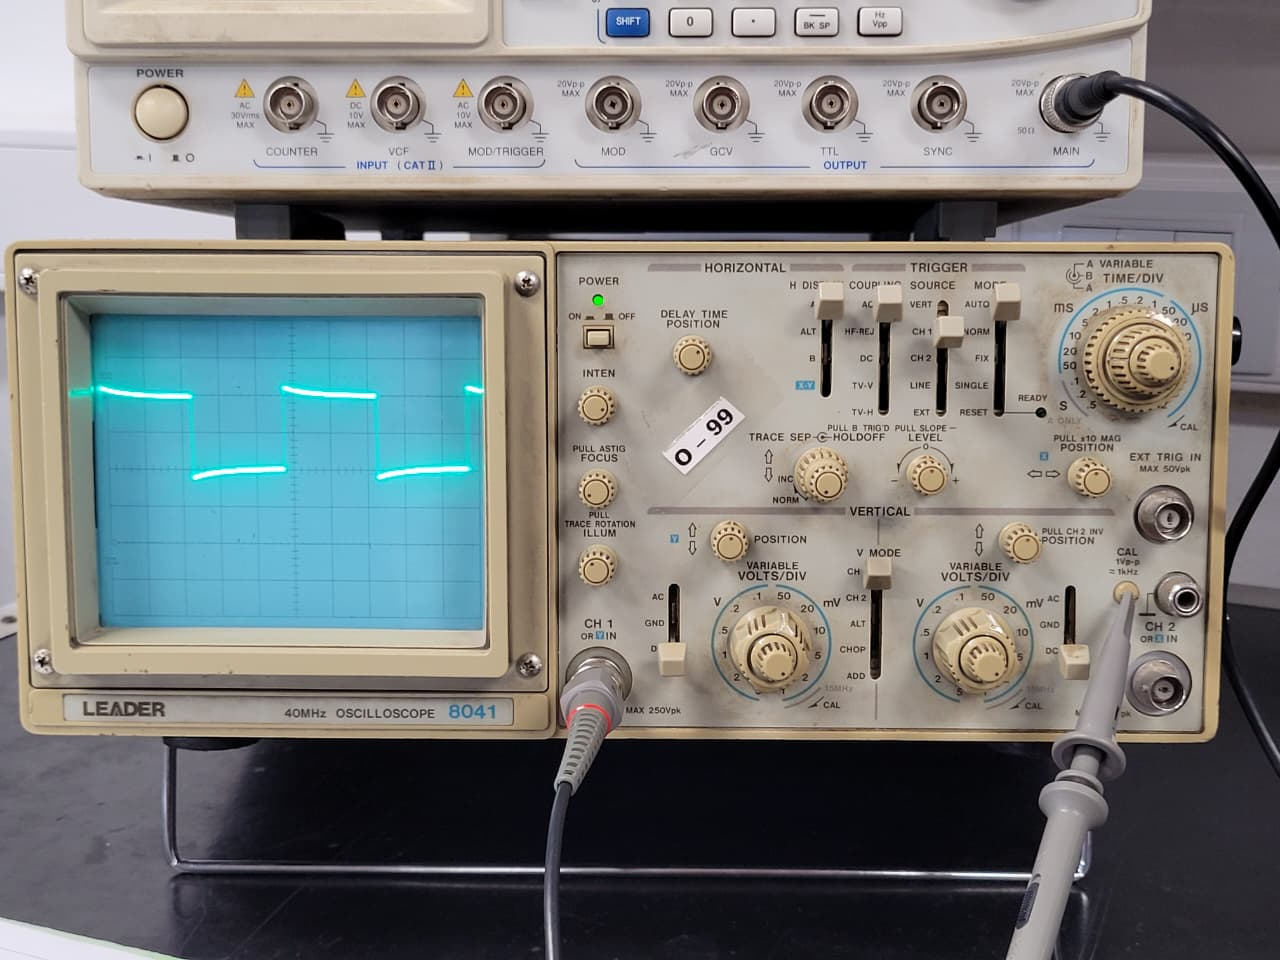
\includegraphics[width=\textwidth]{pictures/osc_1a_cuadrada.jpeg}
        \caption{Exceso}
    \end{subfigure}
    \hfill
    \begin{subfigure}[b]{0.3\textwidth}
        \centering
        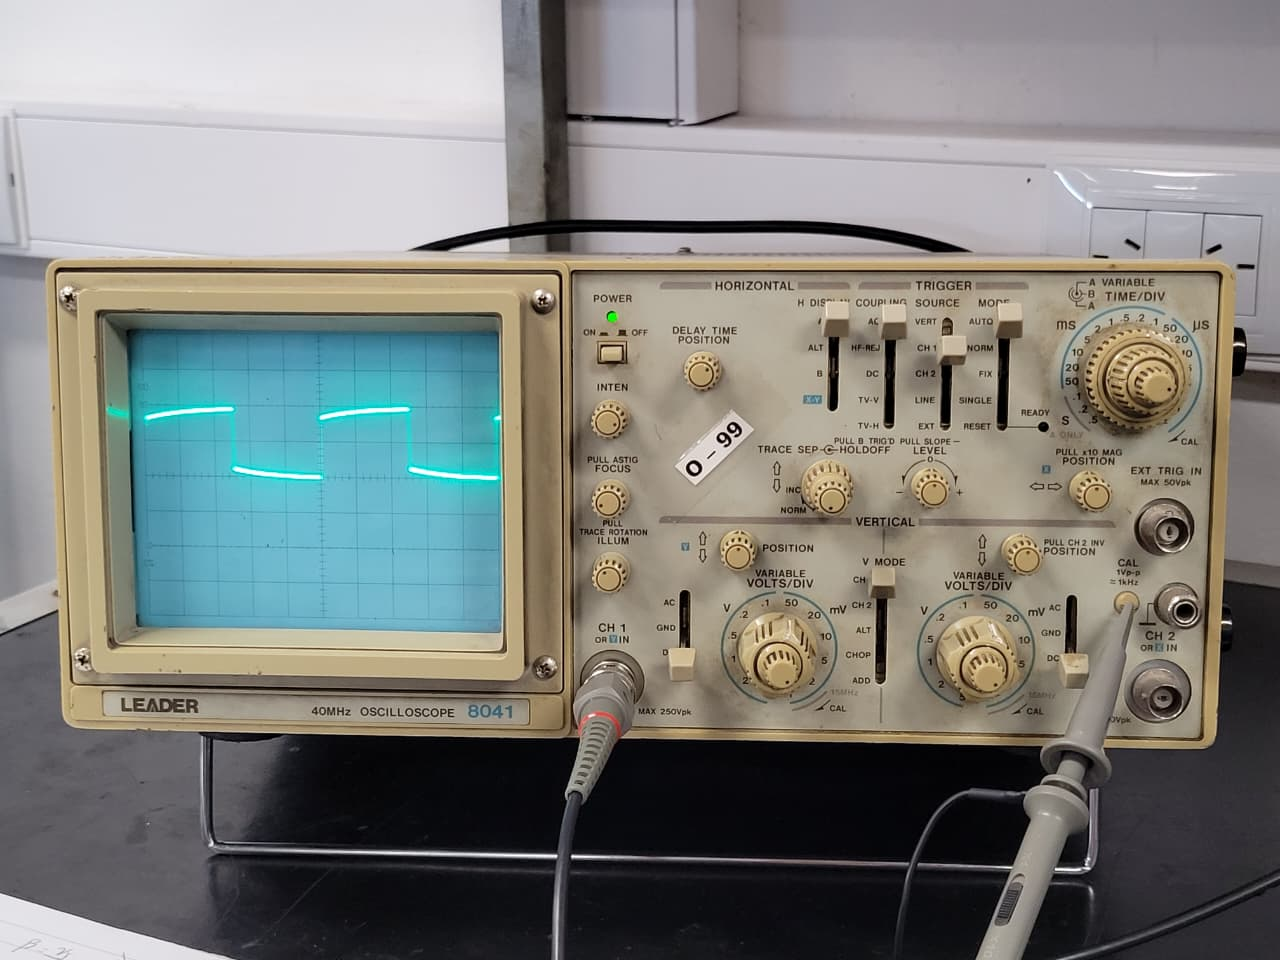
\includegraphics[width=\textwidth]{pictures/osc_1b_cuadrada.jpeg}
        \caption{Defecto}
    \end{subfigure}
    \hfill
    \begin{subfigure}[b]{0.3\textwidth}
        \centering
        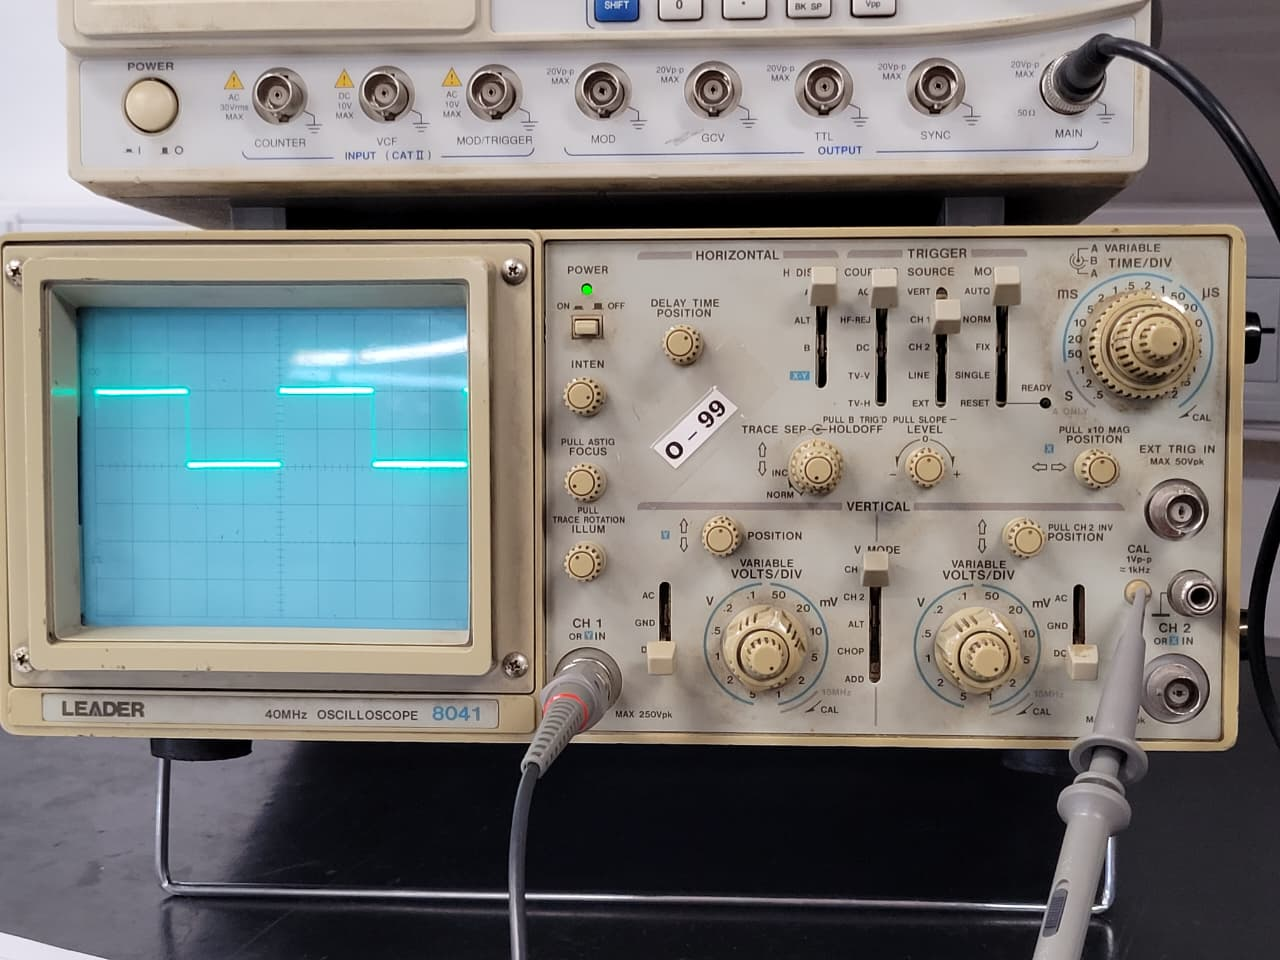
\includegraphics[width=\textwidth]{pictures/osc_1c_cuadrada.jpeg}
        \caption{Compensada}
    \end{subfigure}
    \caption{Estados de compensación de la punta.}
\end{figure}

Para evidenciar la diferencia en la atenuación y distorsión de la señal a distintas frecuencias, se capturaron
oscilogramas a \qty{100}{Hz} y \qty{1}{MHz} para cada estado de compensación de la punta:

\begin{figure}[!ht]
    \centering
    \begin{subfigure}[b]{0.3\textwidth}
        \centering
        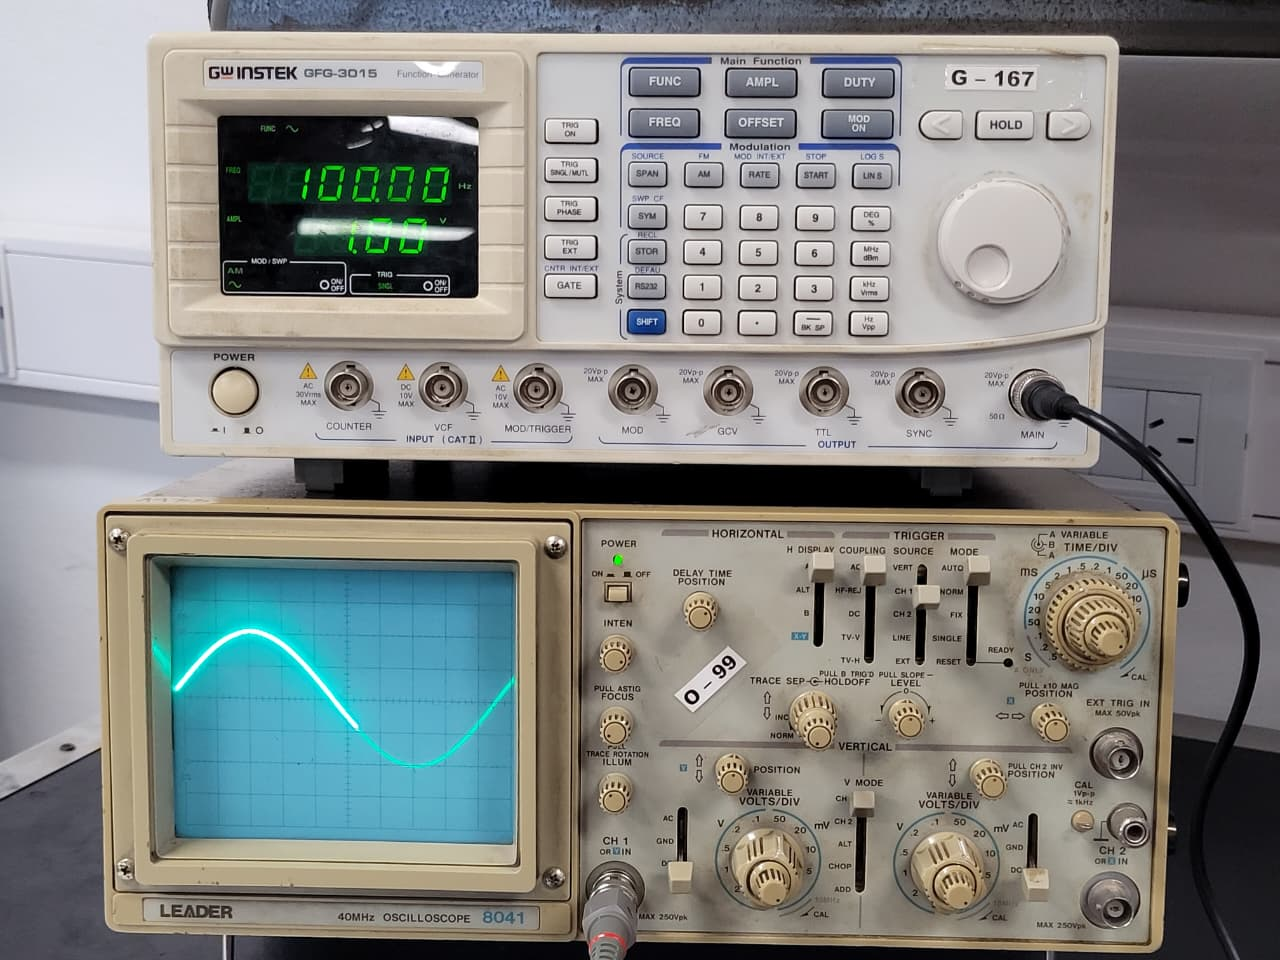
\includegraphics[width=\textwidth]{pictures/osc_1a_100hz.jpeg}
        \caption{Exceso}
    \end{subfigure}
    \hfill
    \begin{subfigure}[b]{0.3\textwidth}
        \centering
        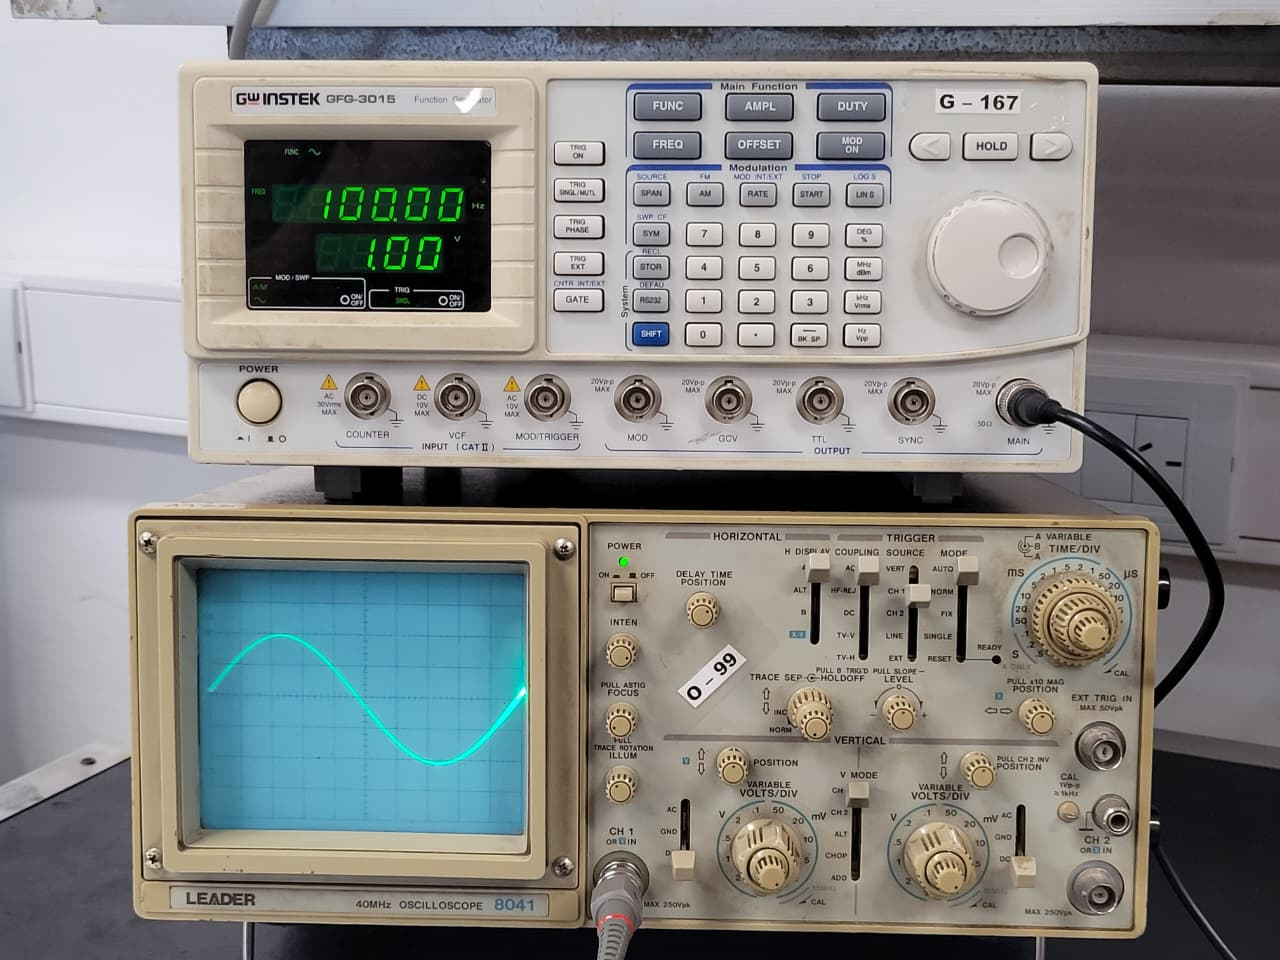
\includegraphics[width=\textwidth]{pictures/osc_1b_100hz.jpeg}
        \caption{Defecto}
    \end{subfigure}
    \hfill
    \begin{subfigure}[b]{0.3\textwidth}
        \centering
        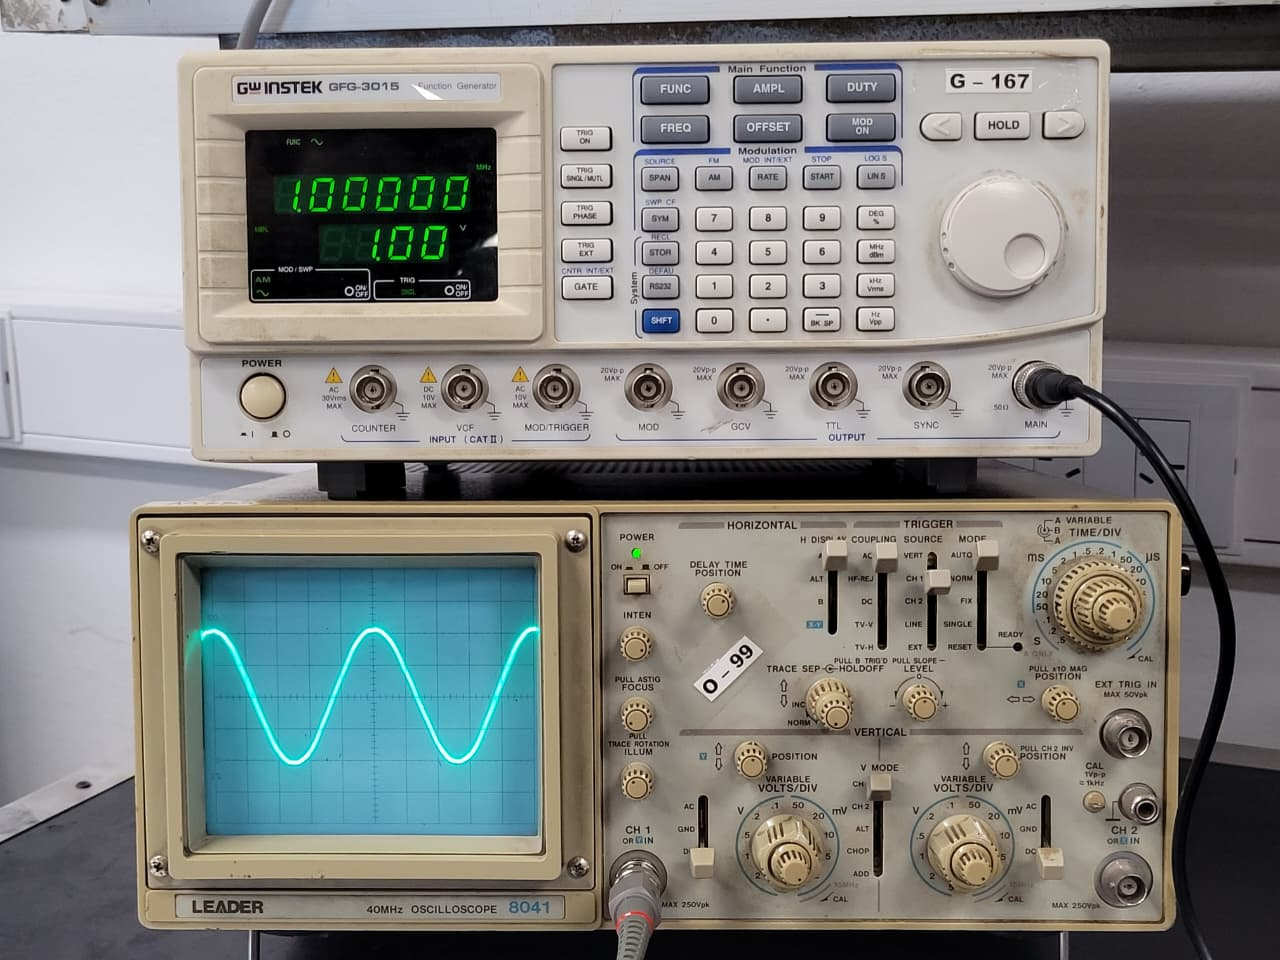
\includegraphics[width=\textwidth]{pictures/osc_1c_100hz.jpeg}
        \caption{Compensada}
    \end{subfigure}
    \caption{Respuesta de la punta a \qty{100}{Hz}.}
\end{figure}

\begin{figure}[H]
    \centering
    \begin{subfigure}[b]{0.3\textwidth}
        \centering
        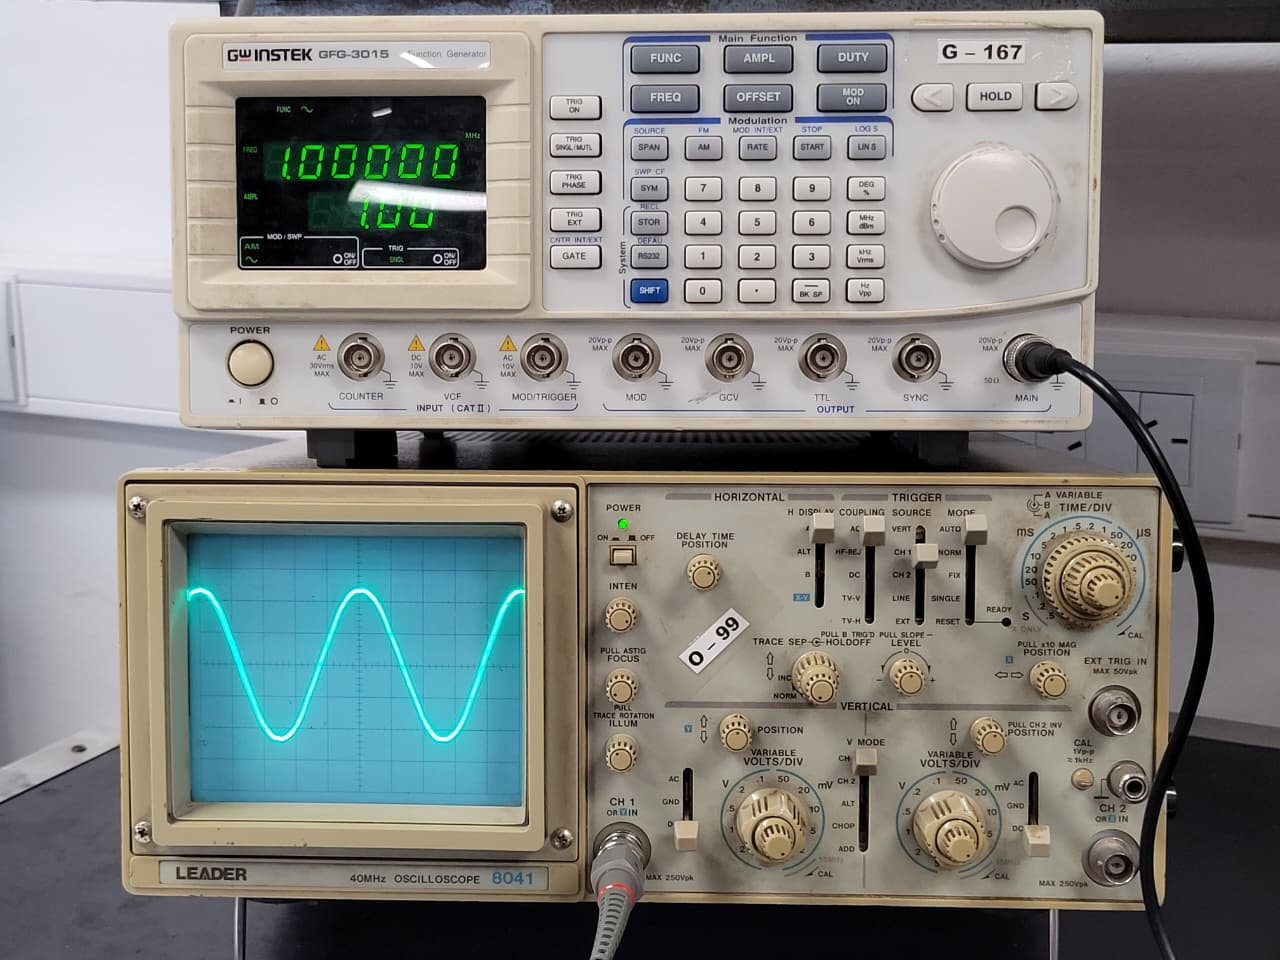
\includegraphics[width=\textwidth]{pictures/osc_1a_1MHz.jpeg}
        \caption{Exceso}
    \end{subfigure}
    \hfill
    \begin{subfigure}[b]{0.3\textwidth}
        \centering
        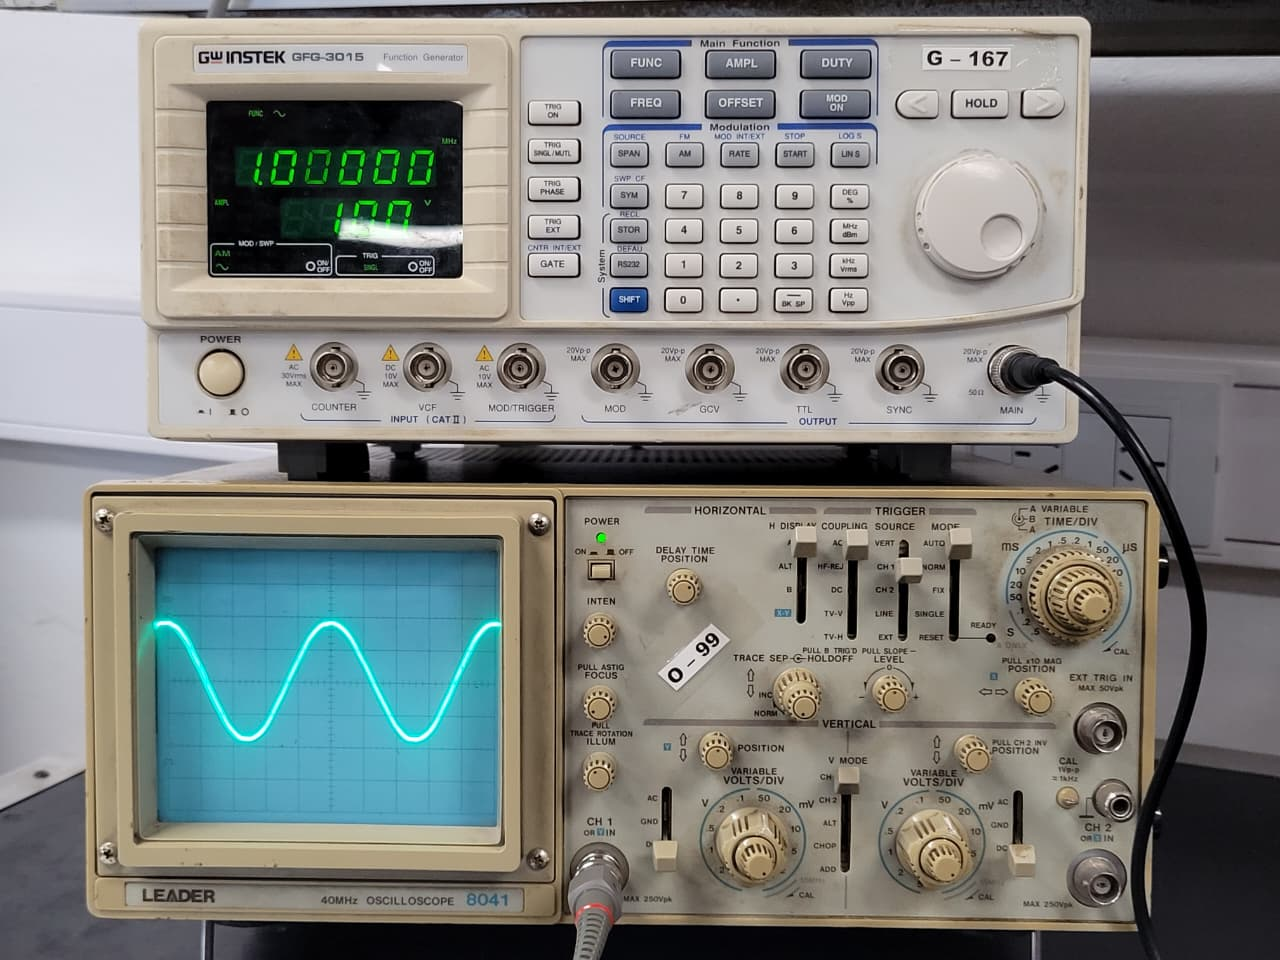
\includegraphics[width=\textwidth]{pictures/osc_1b_1MHz.jpeg}
        \caption{Defecto}
    \end{subfigure}
    \hfill
    \begin{subfigure}[b]{0.3\textwidth}
        \centering
        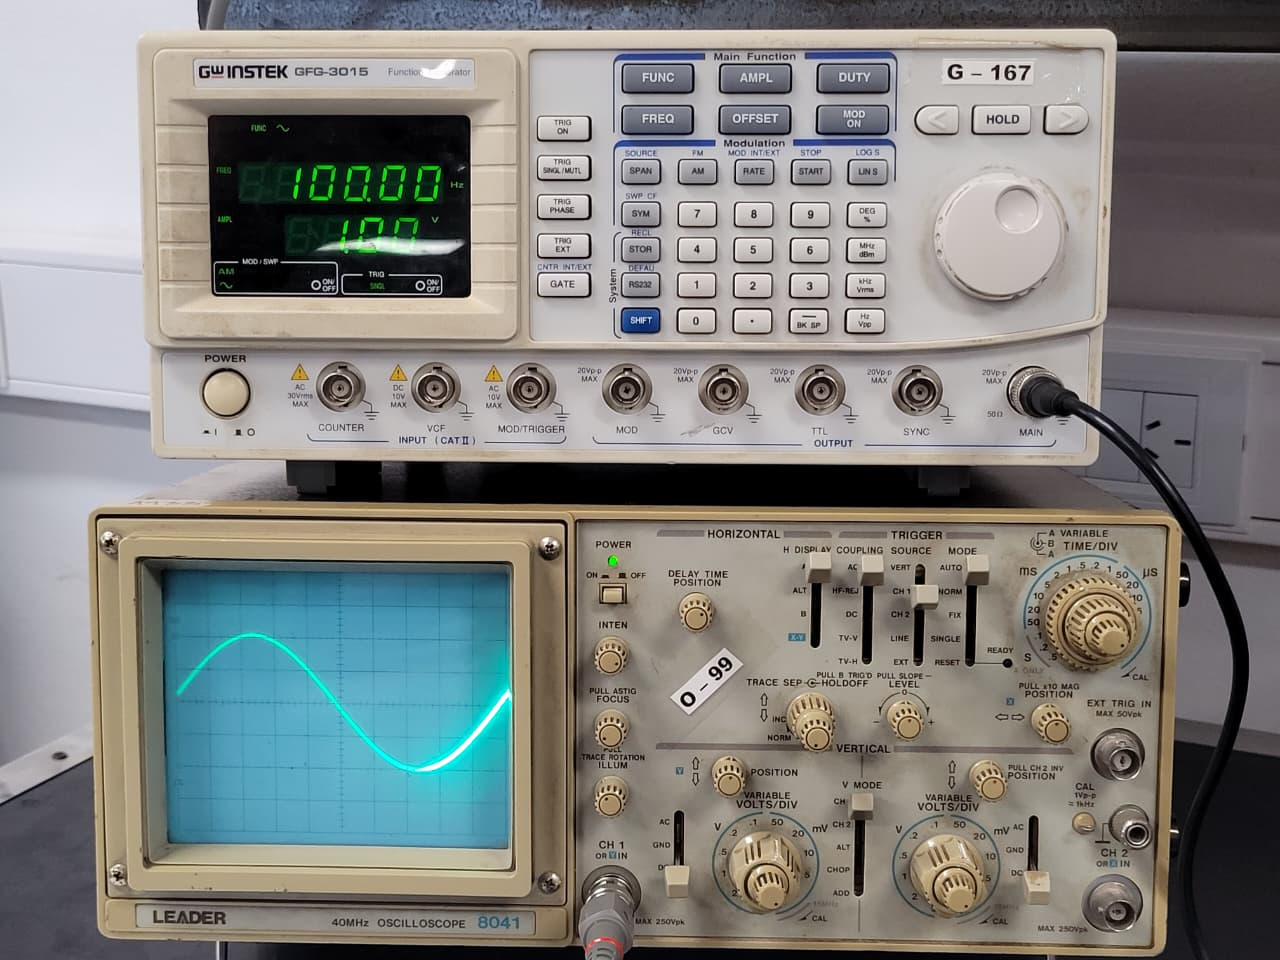
\includegraphics[width=\textwidth]{pictures/osc_1c_1MHz.jpeg}
        \caption{Compensada}
    \end{subfigure}
    \caption{Respuesta de la punta a \qty{1}{MHz}.}
\end{figure}

A continuación se muestra la respuesta en frecuencia de la punta para diferentes estados de compensación:

\begin{table}[!ht]
    \centering
    \begin{tabular}{|c|c|c|c|}
        \hline
        \textbf{f [Hz]} & \textbf{$A_a$ [Vpp]} & \textbf{$A_b$ [Vpp]} & \textbf{$A_c$ [Vpp]} \\ \hline
        100   & \qty{200}{mV} & \qty{200}{mV} & \qty{200}{mV} \\ \hline
        500   & \qty{210}{mV} & "             & \qty{205}{mV} \\ \hline
        1k    & \qty{215}{mV} & \qty{190}{mV} & "             \\ \hline
        5k    & \qty{230}{mV} & \qty{180}{mV} & "             \\ \hline
        10k   & "             & "             & "             \\ \hline
        50k   & "             & "             & "             \\ \hline
        100k  & "             & "             & "             \\ \hline
        300k  & "             & "             & "             \\ \hline
        1M    & "             & "             & "             \\ \hline
    \end{tabular}
    \caption{Respuesta en frecuencia para diferentes compensaciones.}
\end{table}

\begin{itemize}
    \item El oscilograma (b) corresponde a ``caída de respuesta en frecuencias elevadas''.
    \item El oscilograma (a) corresponde a ``exceso de respuesta en frecuencias elevadas''.
    \item El oscilograma (c) corresponde a ``respuesta plana''.
\end{itemize}


\section{Experiencia 2: Acoplamiento CC/CA de la entrada vertical}
Se observó el efecto del capacitor de bloqueo en señales de baja frecuencia (\qty{50}{Hz}). Con atenuación X10 en DC y AC, no hubo variación notable.

\cuadrocontroles{\qty{5}{V}}{-}{-}{X1}{-}

\begin{figure}[!ht]
    \centering
    \begin{subfigure}[b]{0.45\textwidth}
        \centering
        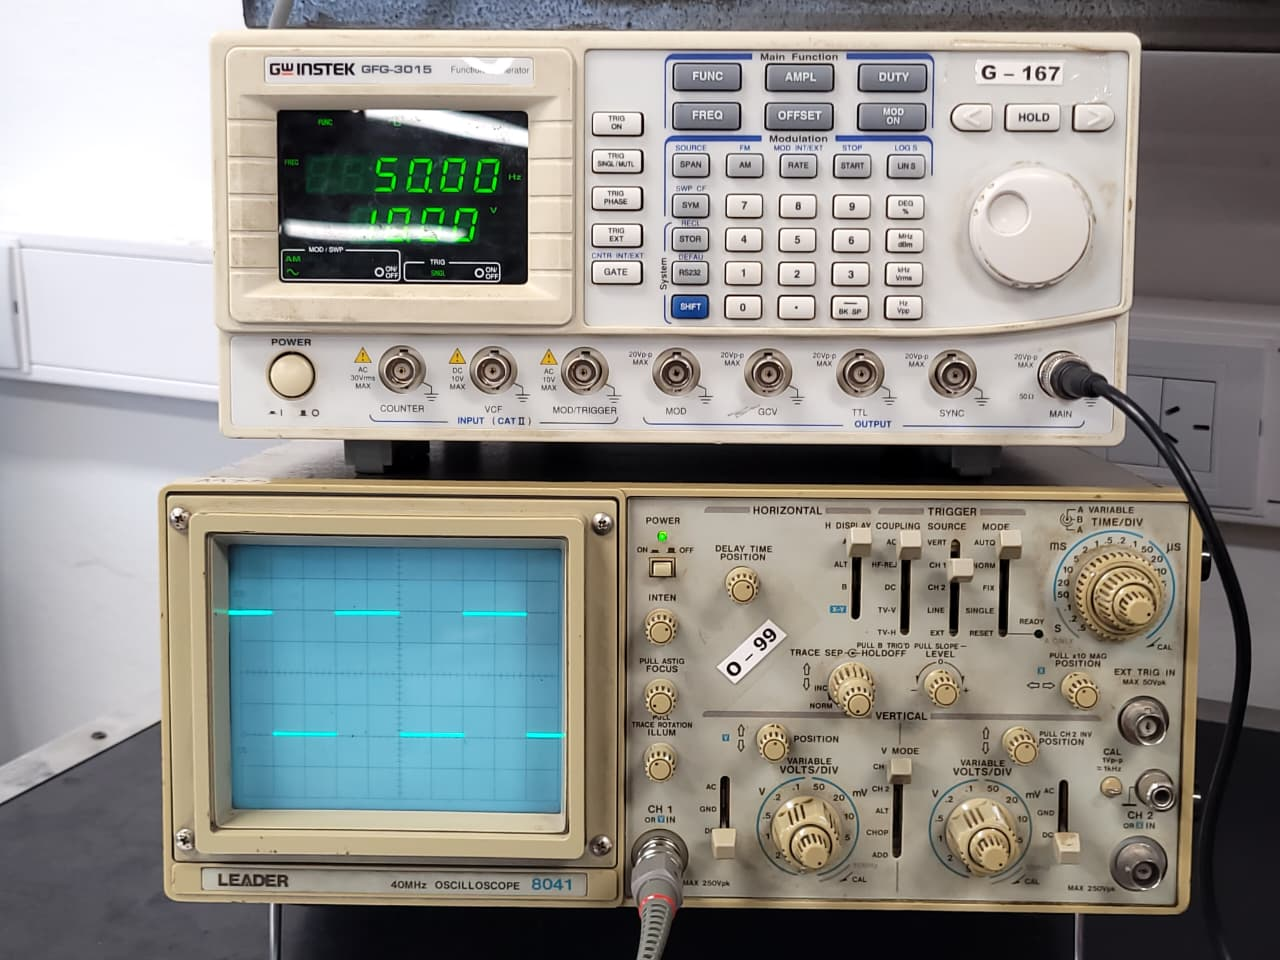
\includegraphics[width=\textwidth]{pictures/osc_2_cc.jpeg}
        \caption{Acoplamiento DC}
    \end{subfigure}
    \hfill
    \begin{subfigure}[b]{0.45\textwidth}
        \centering
        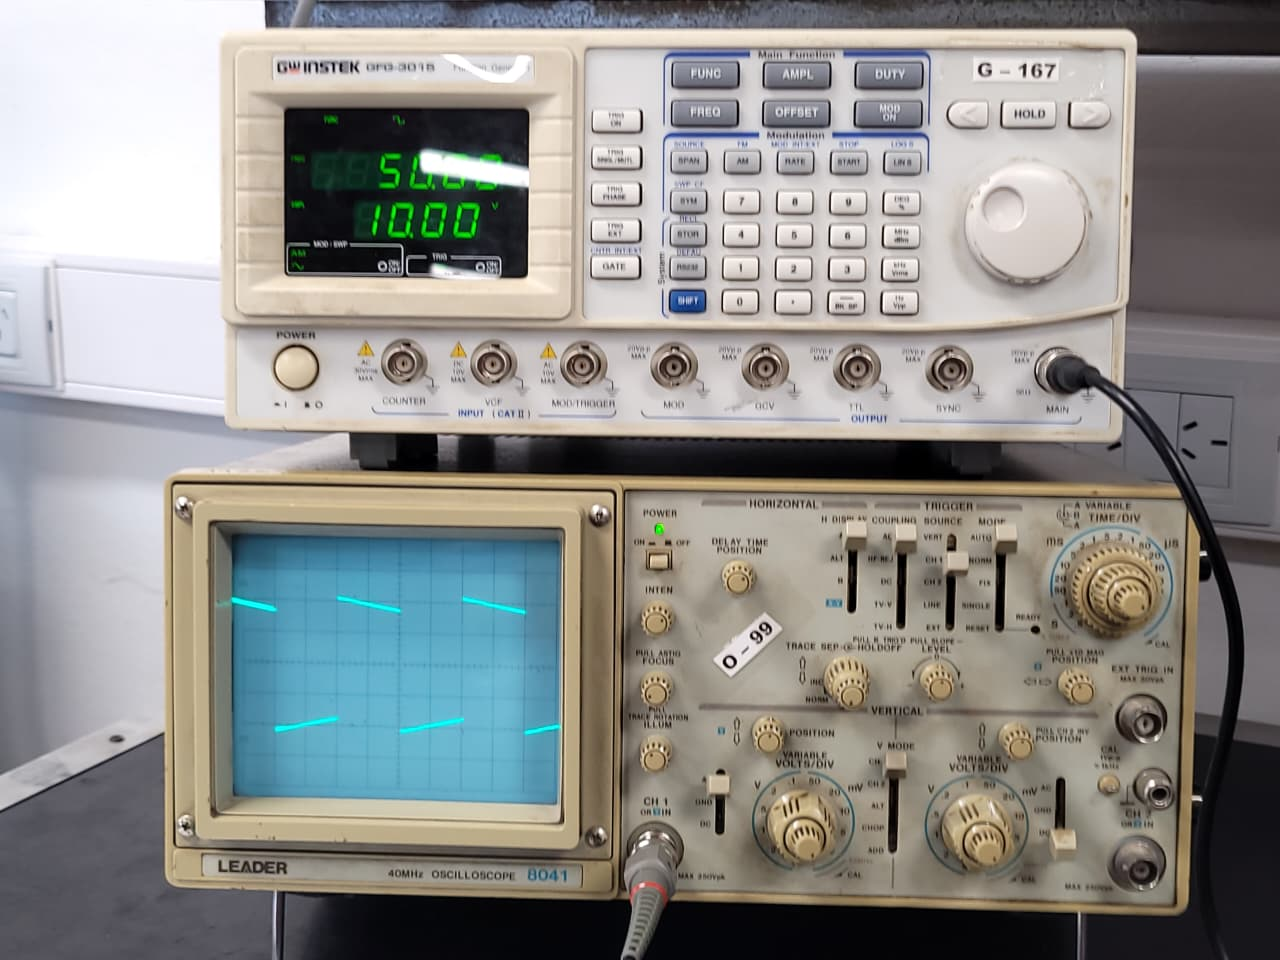
\includegraphics[width=\textwidth]{pictures/osc_2_ca.jpeg}
        \caption{Acoplamiento AC}
    \end{subfigure}
    \caption{Efecto del acoplamiento en la entrada vertical.}
\end{figure}

\section{Experiencia 3: Medición de Vcc y Ripple - Disparo por Línea}
Se midió la tensión de salida de una fuente.
\begin{itemize}
    \item $V_{CC}$ (no reg): \qty{22.5}{V}
    \item $V_{ripple}$ (pp): \qty{1.83}{V}
    \item $f_{ripple}$: \qty{100}{Hz}
    \item Porcentaje de ripple: \qty{8.2}{\%} respecto a $V_{CC}$.
\end{itemize}

\cuadrocontroles{\qty{500}{mV}}{-}{\qty{5}{ms}}{X10}{-}
\begin{figure}[!ht]
    \centering
    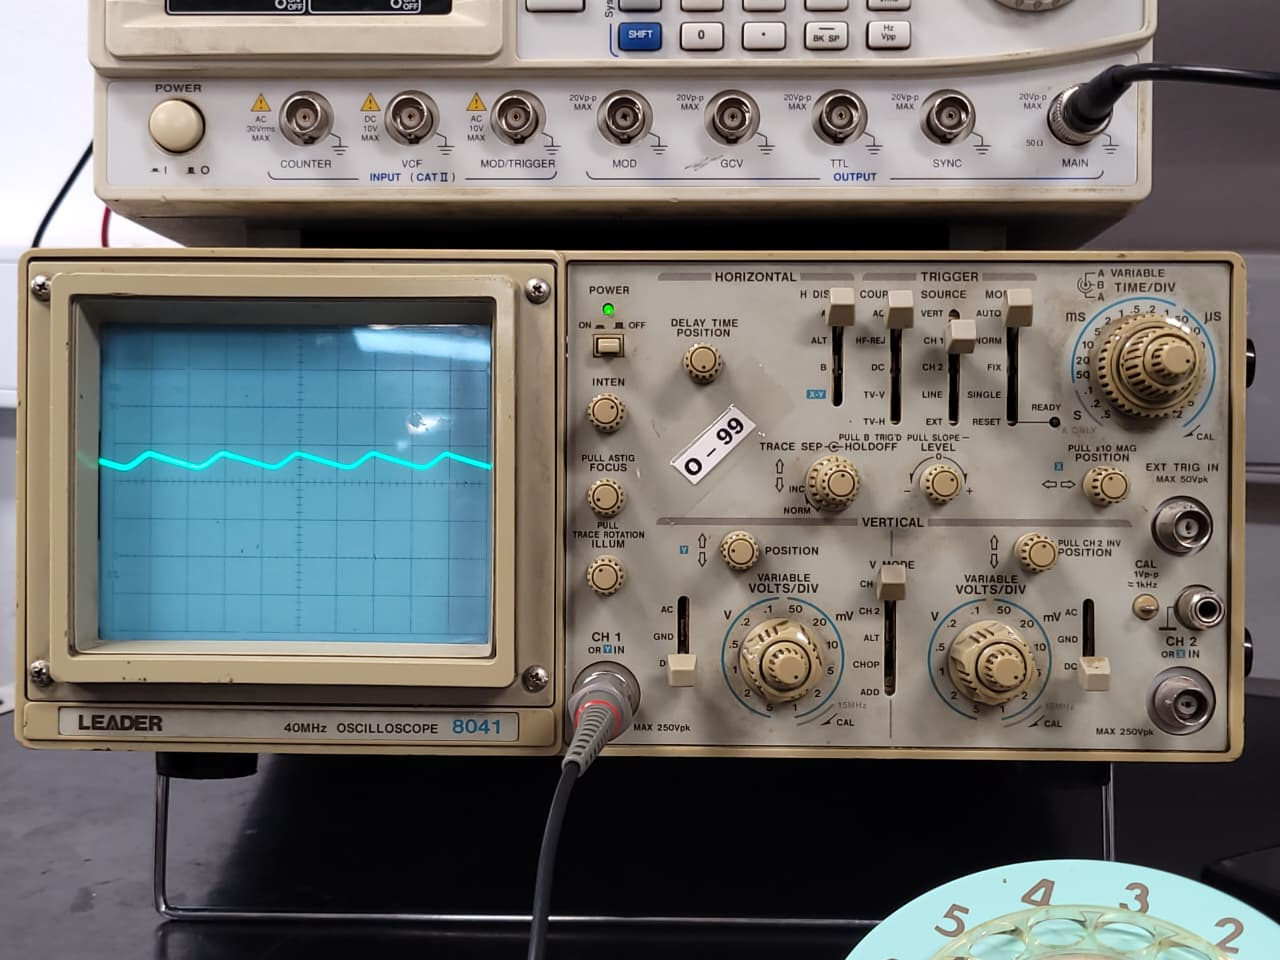
\includegraphics[width=0.6\textwidth]{pictures/osc_3_vcc.jpeg}
    \caption{Medición de componente continua ($V_{CC}$).}
\end{figure}

\cuadrocontroles{\qty{50}{mV}}{-}{\qty{2}{ms}}{X10}{-}
\begin{figure}[!ht]
    \centering
    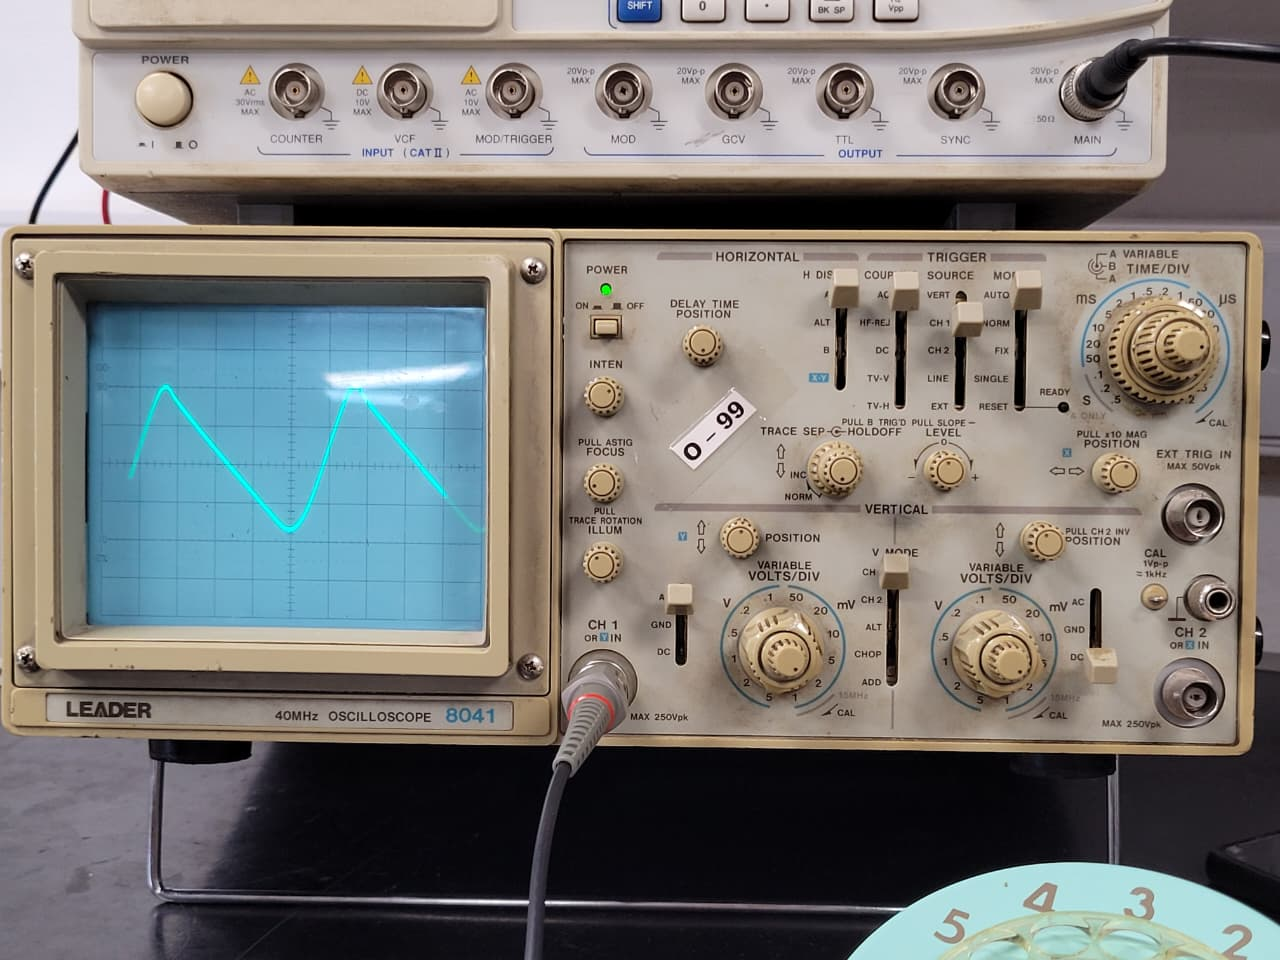
\includegraphics[width=0.6\textwidth]{pictures/osc_3_ripple.jpeg}
    \caption{Medición de ripple superpuesto.}
\end{figure}

\section{Experiencia 4 y 5: Disparo Interno y Externo}
Se analizó el funcionamiento del trigger. El nivel mínimo de señal que activa el trigger es de 0.1 divisiones o \qty{2}{V/div} (con atenuación X1).

\cuadrocontroles{\qty{20}{mV}}{-}{\qty{0.5}{ms}}{X1}{-}
\begin{figure}[!ht]
    \centering
    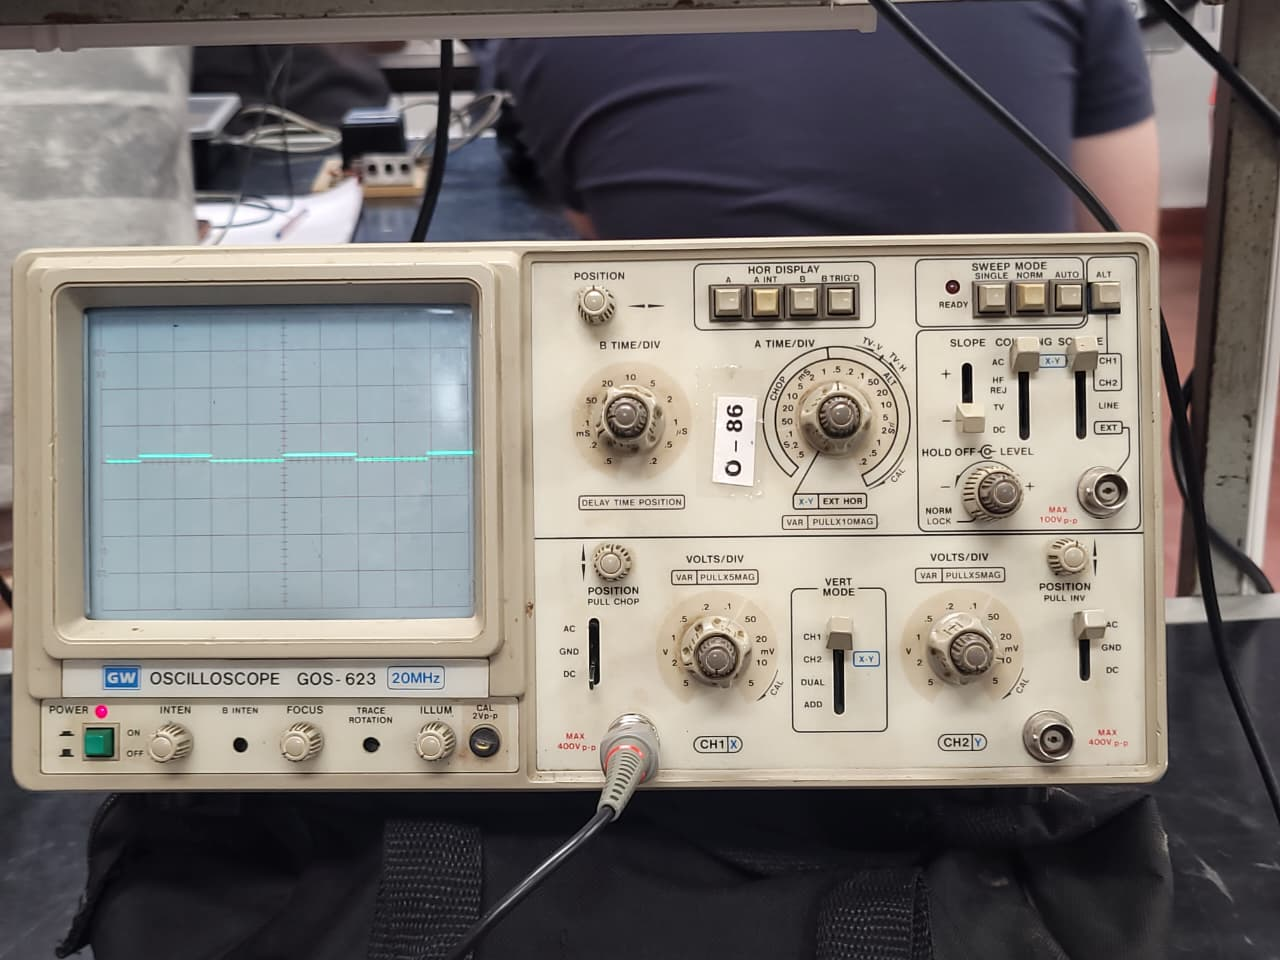
\includegraphics[width=0.6\textwidth]{pictures/osc_4.jpeg}
    \caption{Sincronismo con disparo interno.}
\end{figure}

Para el disparo externo, se obtuvo una frecuencia de \qty{600}{Hz} con $V_{pp} = \qty{200}{mV}$.
\begin{figure}[!ht]
    \centering
    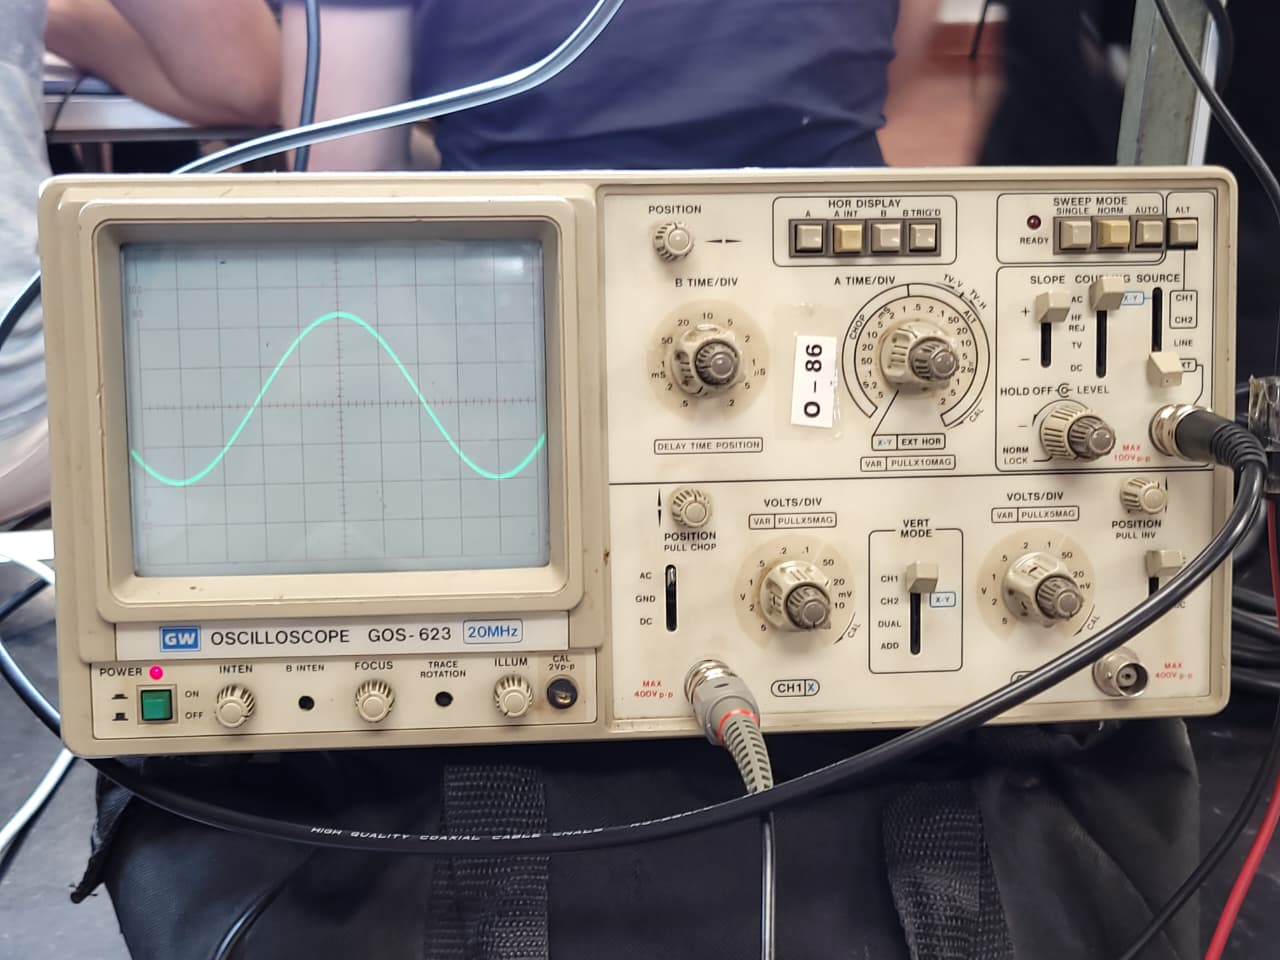
\includegraphics[width=0.6\textwidth]{pictures/osc_5.jpeg}
    \caption{Sincronismo con disparo externo (SYNC).}
\end{figure}

\section{Experiencia 6: Modo X-Y y Figuras de Lissajous}
Se determinó la frecuencia de un generador desconocido.
\begin{itemize}
    \item Frecuencia: \qty{400}{Hz}
    \item $V_{pp}$: \qty{1.1}{V}
\end{itemize}

\cuadrocontroles{\qty{0.2}{V}}{-}{\qty{0.5}{ms}}{X10}{-}
\begin{figure}[!ht]
    \centering
    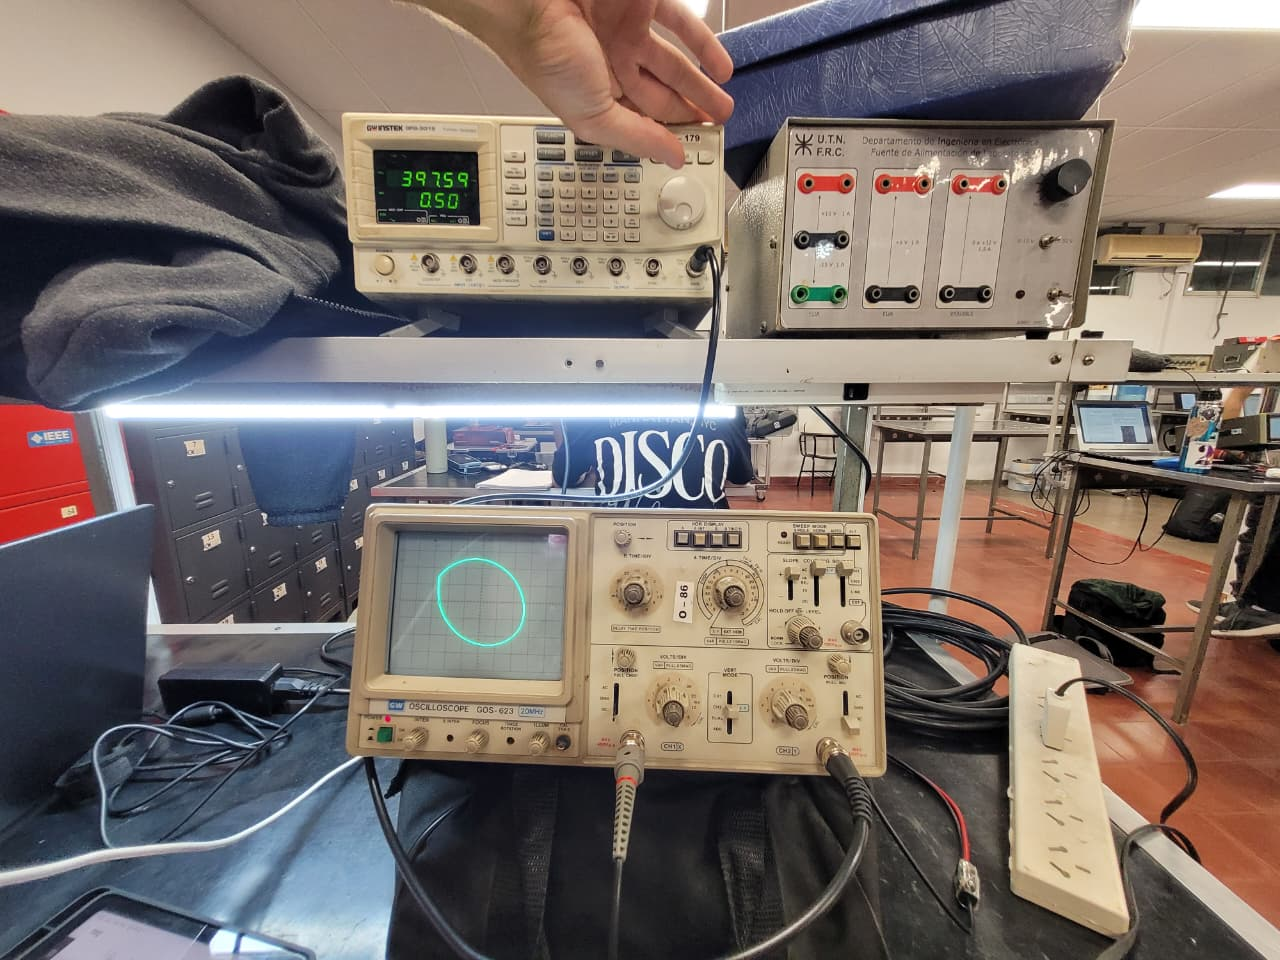
\includegraphics[width=0.6\textwidth]{pictures/osc_6_xy.jpeg}
    \caption{Figura de Lissajous en modo X-Y.}
\end{figure}

\section{Experiencia 7: Uso del Hold-off}
Se utilizó el control de hold-off para estabilizar un tren de pulsos dobles.

\cuadrocontroles{\qty{0.1}{V}}{-}{\qty{0.5}{ms}}{X10}{-}
\begin{figure}[!ht]
    \centering
    \begin{subfigure}[b]{0.45\textwidth}
        \centering
        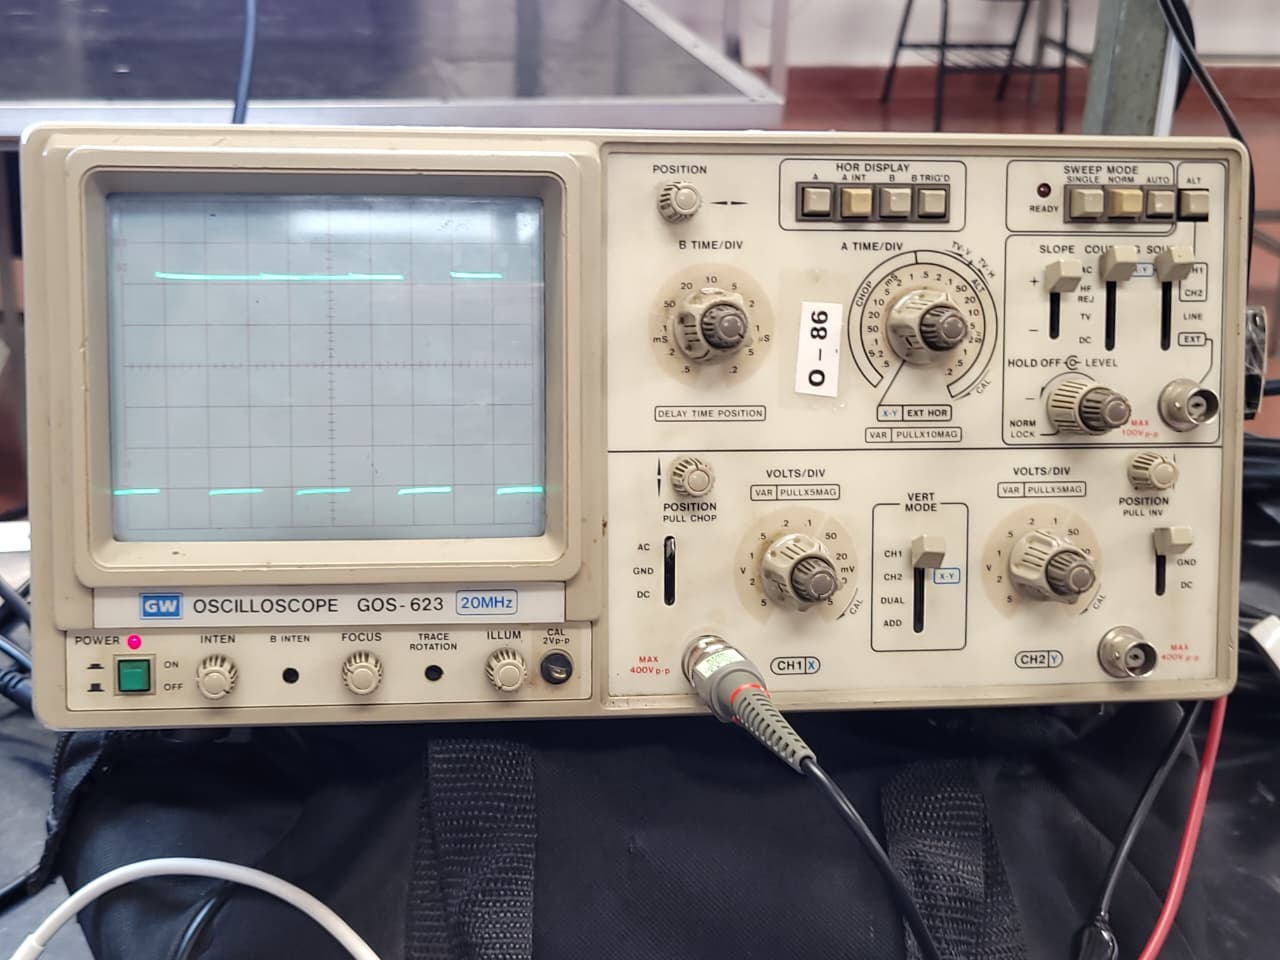
\includegraphics[width=\textwidth]{pictures/osc_7_noholdoff.jpeg}
        \caption{Sin Hold-off}
    \end{subfigure}
    \hfill
    \begin{subfigure}[b]{0.45\textwidth}
        \centering
        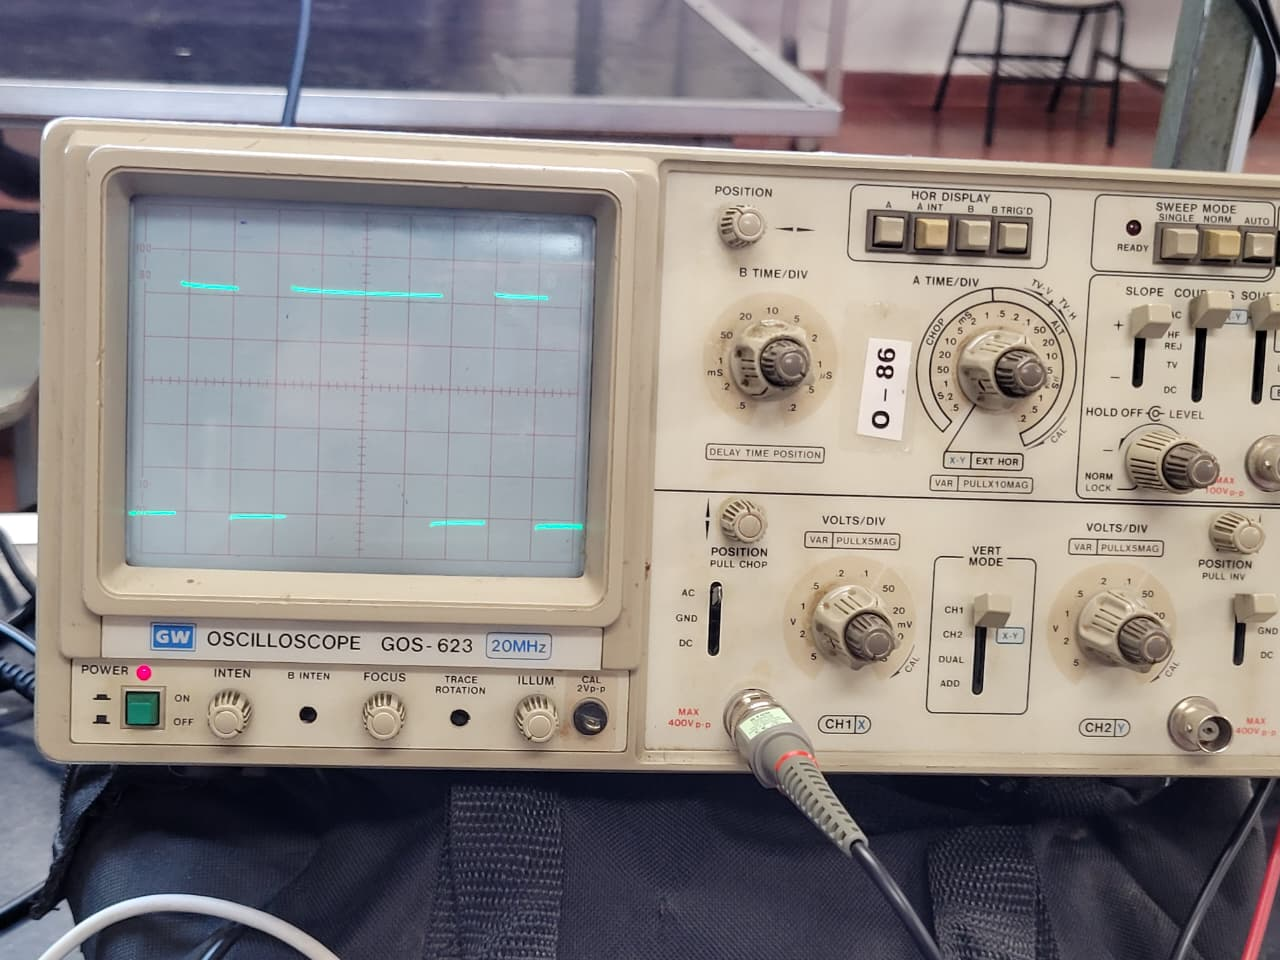
\includegraphics[width=\textwidth]{pictures/osc_7_holdoff.jpeg}
        \caption{Con Hold-off ajustado}
    \end{subfigure}
    \caption{Estabilización de señales complejas mediante Hold-off.}
\end{figure}

\section{Experiencia 8: Modo Doble Trazo}
Se analizó la relación temporal entre las señales MAIN (CH1) y MOD (CH2).

\cuadrocontroles{\qty{0.1}{V}}{\qty{1}{V}}{\qty{0.5}{ms}}{X10}{X1}
\begin{figure}[!ht]
    \centering
    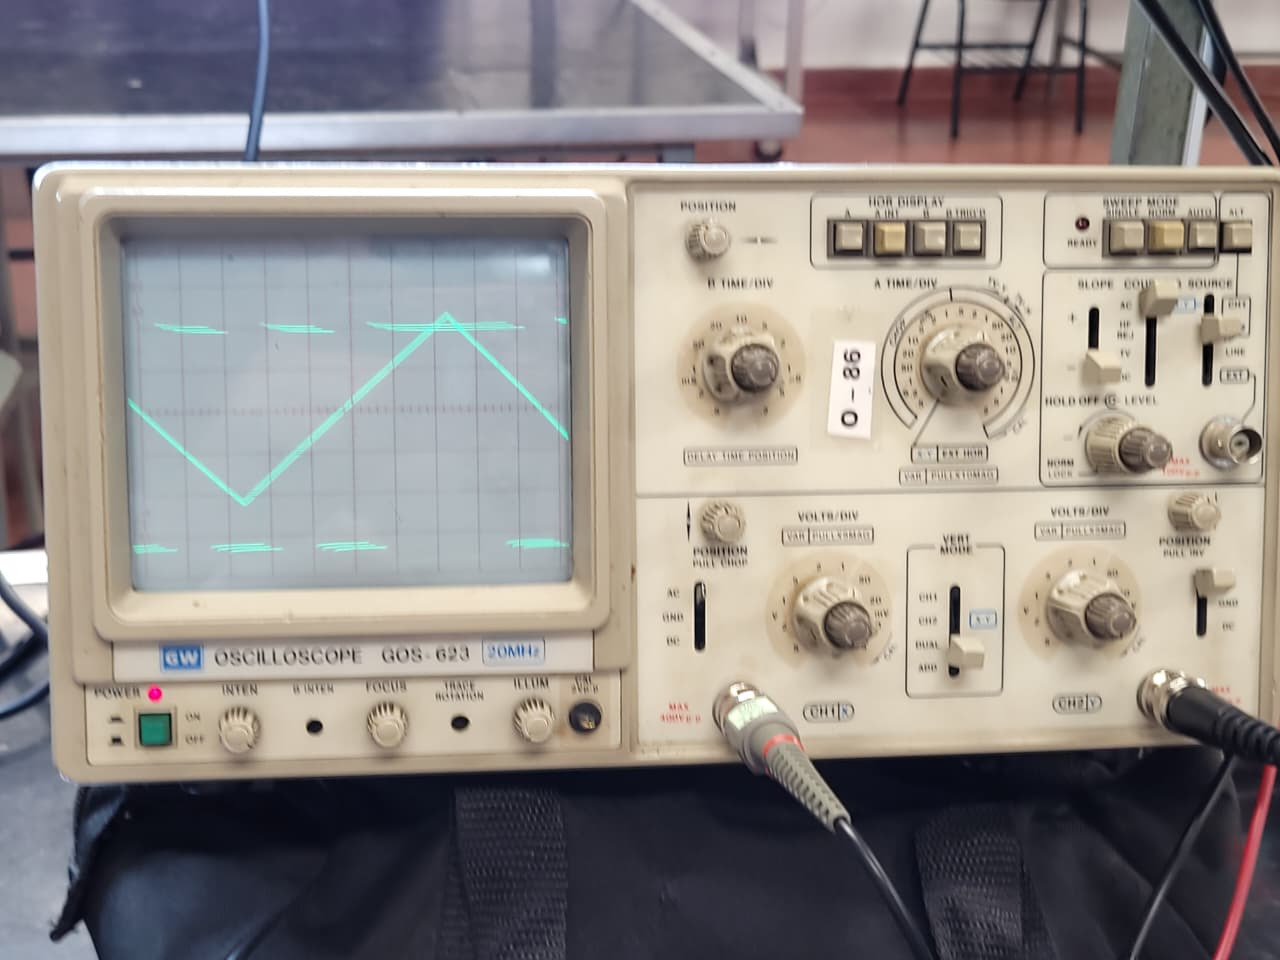
\includegraphics[width=0.6\textwidth]{pictures/osc_8.jpeg}
    \caption{Comparación de señales en modo Dual.}
\end{figure}

\section{Experiencia 9: Filtros de rechazo de la sección de disparo}
Se utilizaron los filtros TV-V y TV-H para estabilizar ráfagas de señal de \qty{15.6}{kHz}.

\cuadrocontroles{\qty{0.1}{V}}{-}{\qty{0.5}{ms}}{X10}{-}
\begin{figure}[!ht]
    \centering
    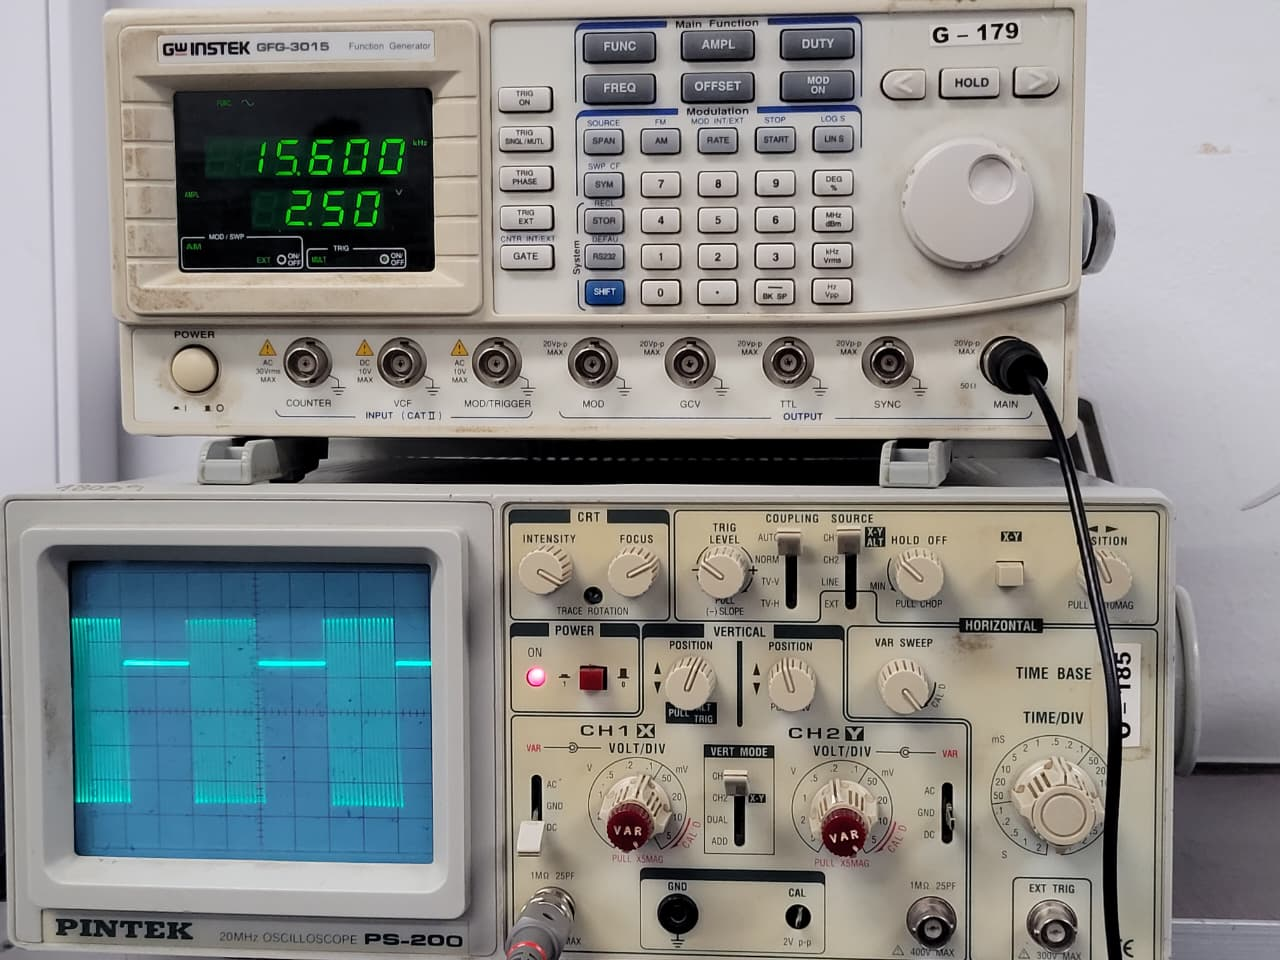
\includegraphics[width=0.6\textwidth]{pictures/osc_9.jpeg}
    \caption{Visualización de ráfaga de señal.}
\end{figure}

\section{Experiencia 10: Función Suma + Canal Invertido}
Se midió una señal diferencial.
\begin{itemize}
    \item Periodo (T): \qty{1}{ms}
    \item Ancho de pulso ($t_o$): \qty{200}{\micro s} (al 50\% de amplitud).
    \item Ciclo de trabajo (D): 0.2
    \item $V_{pp}$: \qty{5.5}{V}
    \item $V_{CC}$: \qty{-2.7}{V}
    \item $V_{ef}$: \qty{2.2}{V} (calculado como $V_{pp} \sqrt{D-D^2}$).
\end{itemize}

\cuadrocontroles{\qty{0.2}{V}}{\qty{0.2}{V}}{\qty{0.2}{ms}}{X10}{X10}
\begin{figure}[!ht]
    \centering
    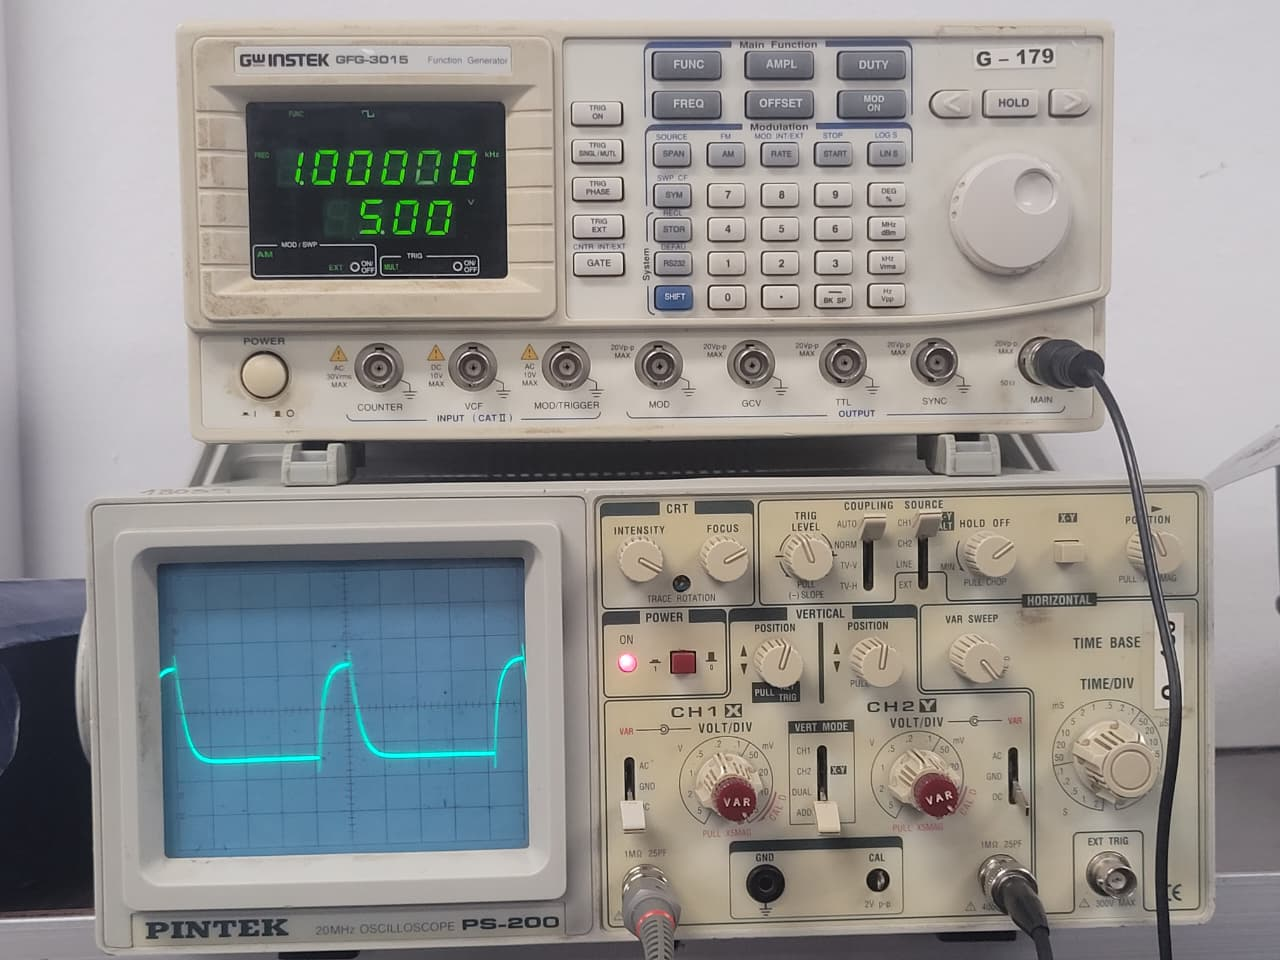
\includegraphics[width=0.6\textwidth]{pictures/osc_10.jpeg}
    \caption{Medición diferencial (ADD + INV).}
\end{figure}

\section{Experiencia 11: Barrido Único y Captura Digital}
Se capturó el tren de pulsos de un disco telefónico.
\begin{itemize}
    \item Duración de los pulsos ($t_o$): \qty{70}{ms}
    \item Periodo de los pulsos (T): \qty{114}{ms}
    \item Demora de silenciamiento ($t_d$): \qty{12}{ms}
\end{itemize}

\begin{figure}[!ht]
    \centering
    \begin{subfigure}[b]{0.45\textwidth}
        \centering
        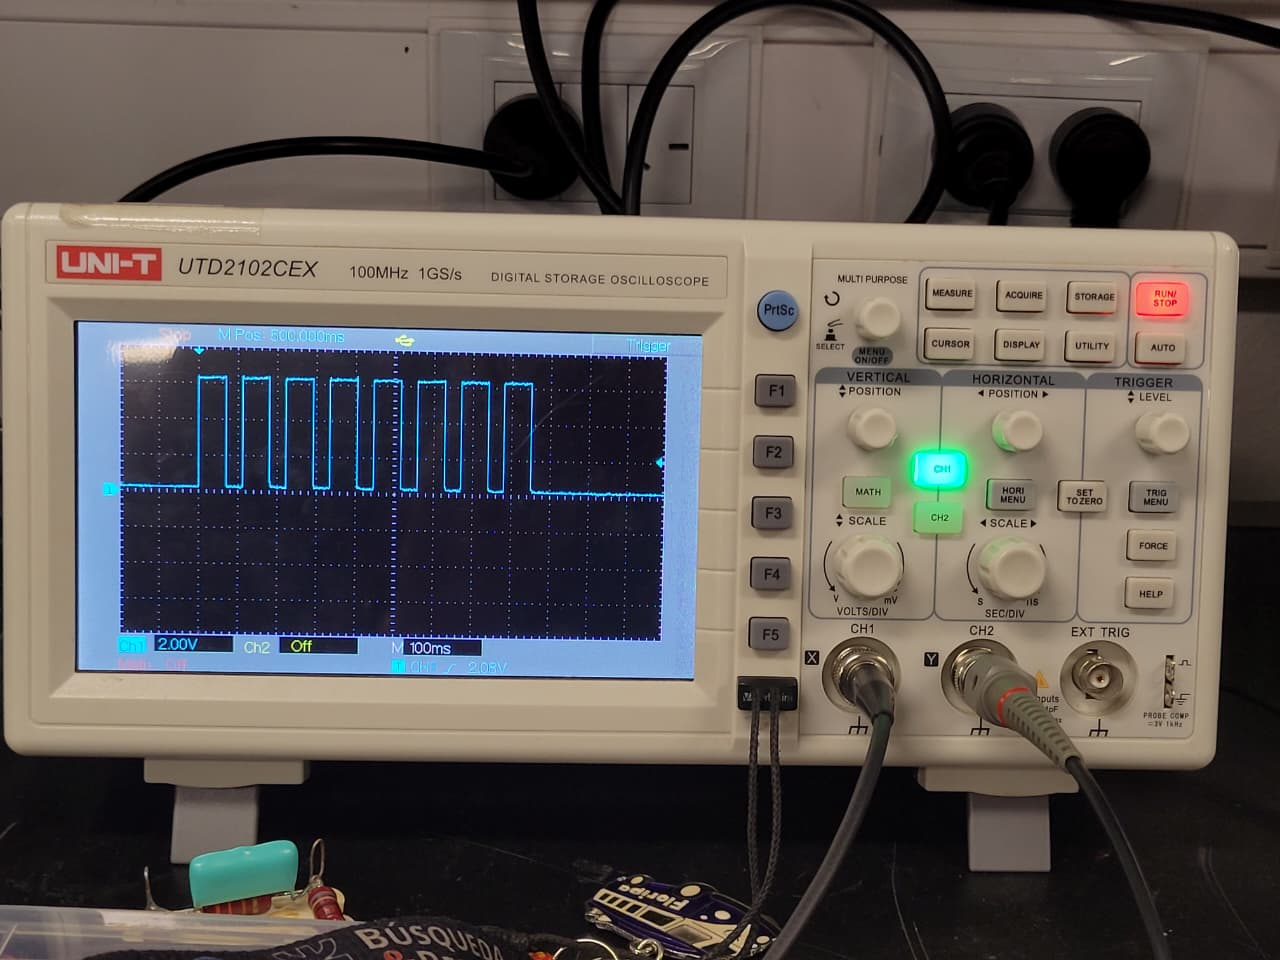
\includegraphics[width=\textwidth]{pictures/11_a.jpeg}
        \caption{Captura del tren de pulsos}
    \end{subfigure}
    \hfill
    \begin{subfigure}[b]{0.45\textwidth}
        \centering
        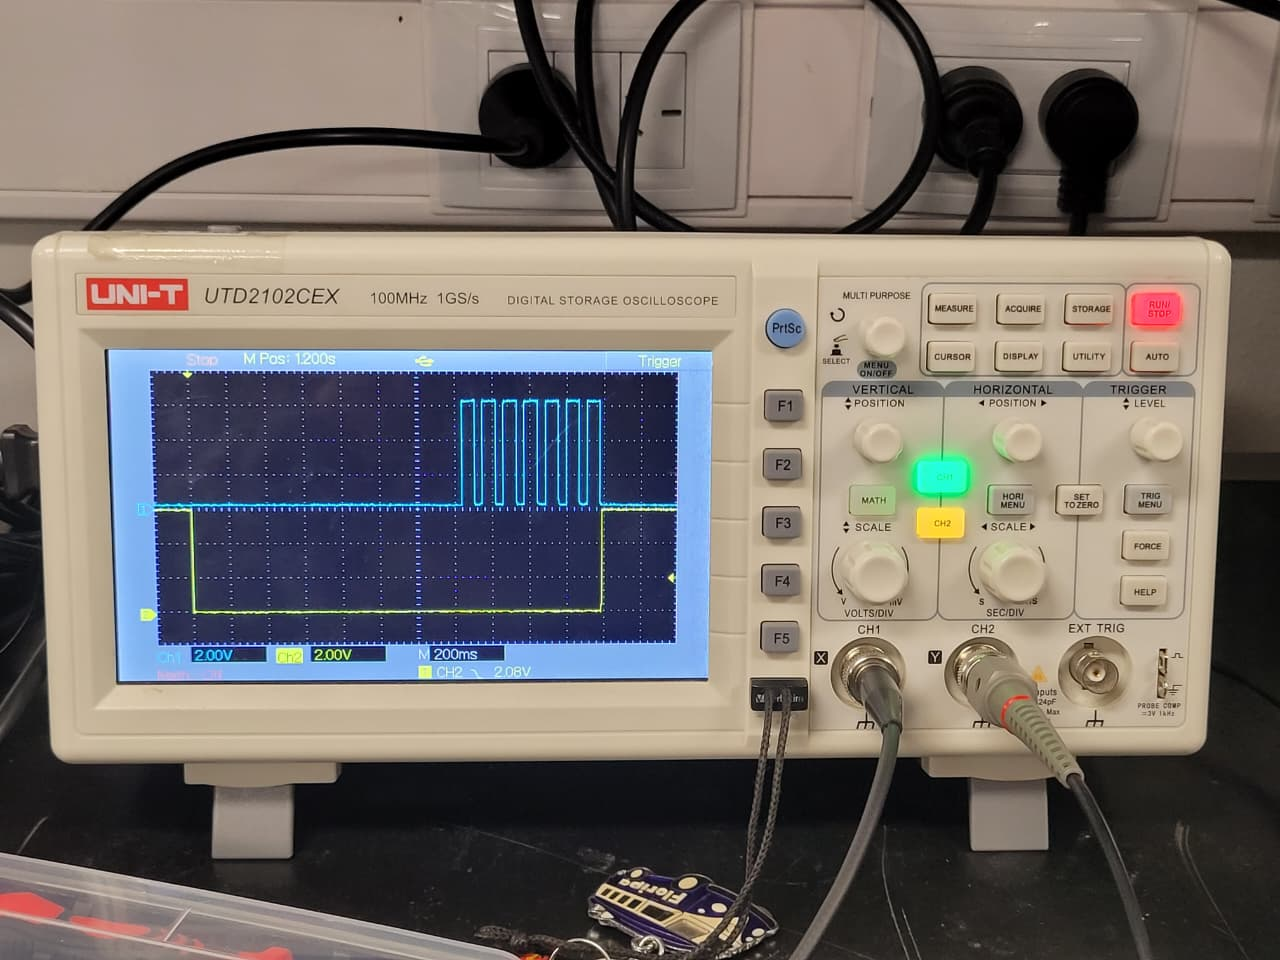
\includegraphics[width=\textwidth]{pictures/11_b.jpeg}
        \caption{Tren de pulsos + Silenciamiento}
    \end{subfigure}
    \caption{Captura de eventos únicos en osciloscopio digital.}
\end{figure}
